%
%===============>>  ГРУППА 10-2 МОДУЛЬ 5  <<=============
%
\setmodule{5}

%BEGIN_FOLD % ====>>_____ Занятие 1 _____<<====
\begin{class}[number=1]
	\begin{definit}
		Сечением фигуры плоскостью является многоугольник, стороны которого принадлежат граням многогранника.
	\end{definit}
	\begin{definit}
		Соединяйте точки, которые лежат в одной грани (в плоскости этой грани).
	\end{definit}
	\begin{definit}
		Плоскость сечения пересекает параллельные грани по параллельным прямым.
	\end{definit}
	\begin{definit}
		Если плоскость сечения проходит через прямую,
		параллельную какой-то плоскости, то секущая плоскость
		пересечёт данную плоскость по параллельной прямой.
	\end{definit}
	\begin{listofex}
		\item Постройте сечение треугольной пирамиды \( DABC \) плоскостью,
		проходящей через следующие точки:
		\begin{tasks}(1)
			\task \( B \), \( D \) и середину \( M \) ребра \( AC \);
			\task середину \( K \) ребра \( AD \) и точки \( L \) и \( M \), лежащие на продолжениях
			рёбер \( AB \) и \( AC \) за точки \( B \) и \( C \);
			\task середины \( K \), \( L \) и \( M \) рёбер AD, AB и BC;
		\end{tasks}
		\item Постройте сечение параллелепипеда \( ABCDA_1B_1C_1D_1 \)
		плоскостью, проходящей через следующие точки:
		\begin{tasks}(1)
			\task середины рёбер \( AB \), \( AD \) и \( AA_1 \);
			\task \( A \), \( C \) и середину ребра \( A_1B_1 \);
			\task середины рёбер \( AA_1 \), \( AD \) и центр грани \( BB_1C_1C \);
			\task середину ребра \( CC_1 \) и точки \( K \), \( L \), лежащие на рёбрах \( AB \) и \( A_1B_1 \),
			если \( BK : KA= A_1L : LB_1=1 : 2 \);
		\end{tasks}
		\item Основание пирамиды \( SABCD \) --- параллелограмм \( ABCD \).
		Постройте сечение пирамиды плоскостью, проходящей через следующие
		точки:
		\begin{tasks}(1)
			\task \( A \), \( B \) и середина ребра \( SD \);
			\task середины рёбер \( AB \), \( BC \) и \( SC \);
			\task середины рёбер \( AB \), \( BC \) и \( SD \);
			\task центр основания, середину ребра \( SD \) и точку \( M \) ребра \( SA \),
			если \( AM : MS = 1 : 3 \);
		\end{tasks}
		\newpage
		\item Основание шестиугольной призмы \( ABCDEFA_1B_1C_1D_1E_1F_1 \) ---
		правильный шестиугольник \( ABCDEF \).
		Постройте сечение призмы плоскостью,
		проходящей через следующие точки:
		\begin{tasks}(1)
			\task \( A \), \( B \) и \( F_1 \);
			\task \( A \), \( C \) и \( D_1 \);
			\task \( B \), \( E \) и середину ребра \( FF_1 \);
			\task \( B \), \( C \) и \( E_1 \);
			\task \( B \), \( D \) и середину ребра \( FF_1 \).
	\end{tasks}
	\end{listofex}
\end{class}
%END_FOLD

%BEGIN_FOLD % ====>>_____ Занятие 2 _____<<====
\begin{class}[number=2]
	\begin{listofex}
		%1
		\item Точка \(M\) лежит на ребре \(AB\) треугольной пирамиды \(ABCD\), причём \(AM : MB = 1:2\). а) Постройте сечение пирамиды плоскостью, проходящей через точку \(M\) и середины рёбер \(BC\) и \(AD\). б) В каком отношении плоскость сечения делит ребро \(CD\)?
		%2
		\item Точка \(M\) — середина ребра \(AD\) треугольной пирамиды \(ABCD\). Точки \(K\) и \(L\) лежат на прямых \(AB\) и \(AC\) соответственно, причём \(B\) --- середина отрезка \(AK\), а \(C\) — середина отрезка \(AL\). а) Постройте сечение пирамиды плоскостью, проходящей через точки \(M, K, L\). б) В каком отношении плоскость сечения делит ребро \(BD\)?
		%3
		\item Точки \(M\) и \(N\) — середины рёбер соответственно \(AB\) и \(BC\) параллелепипеда \(ABCDA_1B_1C_1D_1\).
		а) Постройте сечение параллелепипеда плоскостью, проходящей через точки \(M, N, D_1\). б) В каком отношении плоскость сечения делит ребро \(AA_1\)?
		%4
		\item Точка \(M\) — середина ребра \(CD\) параллелепипеда \(ABCDA_1B_1C_1D_1\). а) Постройте сечение параллелепипеда плоскостью, проходящей через точки \(M, A, C\). б) Пусть секущая плоскость пересекает прямую \(DD_1\) в точке \(P\). Найдите отношение \(PD:PDV\)
		%5
		\item Основание пирамиды \(SABCD\) — параллелограмм \(ABCD\) с центром \(O\). Точка \(M\) лежит на отрезке \(SO\), причём \(OM:MS = 1:2\). а) Постройте сечение пирамиды плоскостью, проходящей через прямую AM параллельно прямой \(BD\). б) В каком отношении плоскость сечения делит ребро \(SC\)?
		%6
		\item Основание пирамиды \(SABCD\) — параллелограмм \(ABCD\) с центром \(O\). Точка \(M\) — середина отрезка \(AO\). а) Постройте сечение пирамиды плоскостью, проходящей через точку \(M\) параллельно прямым \(SA\) и \(BD\). б) В каком отношении плоскость сечения делит ребро \(SC\)?
	\end{listofex}
\end{class}
%END_FOLD

%BEGIN_FOLD % ====>>_____ Занятие 3 _____<<====
\begin{class}[number=3]
	\begin{listofex}
%		\item Основание пирамиды \(SABCD\) --- параллелограмм \(ABCD\). Точка К --- середина ребра \(SD\). а) Плоскость проходит через точку \(K\) параллельно медианам \(BM\) и \(SN\) граней \(BSC\) и \(ASD\). Постройте прямую пересечения этой плоскости с плоскостью основания пирамиды. б) Найдите угол между прямыми \(BM\) и \(SN\), если пирамида \(SABCD\) правильная, причём все её рёбра равны.
%		\item Дан куб \(ABCDA_1B_1C_1D_1\). Найдите угол между плоскостями: а) \(BCC_1\) и \(ABC_1\), б) \(ABC\) и \(CB_1D_1\); в) \(BA_1C_1\) и \(AB_1D_1\); г) \(ABC_1\) и \(BCD_1\).
%		\item Дана правильная четырёхугольная пирамида \(SABCD\) с вершиной \(S\). Все рёбра пирамиды равны, \(E\) — середина бокового ребра \(SC\). Найдите углы между плоскостями: a) \(SAD\) и \(SBC\); б) \(ABC\) и \(SCD\); в) \(ABC\) и \(BDE\); г) \(BSC\) и \(DSC\); д) \(ABE\) и \(ABC\).
%		\item Дана правильная треугольная призма \(ABCA_1B_1C_1\). Боковое ребро \(AA_1\)) равно стороне основания \(ABC\). Точка \(M\) — середина ребра \(BC\). Найдите углы между плоскостями: а) \(AA_1M\) и \(ABC\); б) \(ABC\) и \(CA_1B_1\); в) \(ACB_1\) и \(BA_1C_1\); г) \(A_1C_1M\) и \(A_1B_1C_1\).
		\item Точки \( M \) и \( N \) --- середины рёбер соответственно \( AB \) и \( CD \) треугольной пирамиды \( DABC \).
		Постройте сечение пирамиды плоскостью, проходящей через середину ребра \( AD \) параллельно прямым \( AB \) и \( CD \).
		В каком отношении плоскость сечения делит отрезок MN?
		\item Точка \( M \) --- середина ребра \( AB \) треугольной призмы \( ABCA_1B_1C_1 \).
		Постройте сечение призмы плоскостью,
		проходящей через прямую \( A_1M \) параллельно прямой \( AC \).
		\item Основания шестиугольной призмы \( ABCDEFA_1B_1C_1E_1F_1 \) --- правильные шестиугольники.
		Точка \( M \) --- середина ребра \( CC_1 \),
		\( O \) --- центр грани \( ABCDEF \).
		Постройте сечение призмы плоскостью, проходящей через
		точки \( M \), \( O \) и \( E_1 \).
		В каком отношении плоскость сечения делит ребро \(EF\)?
	\end{listofex}
\end{class}
%END_FOLD

%BEGIN_FOLD % ====>>_____ Занятие 4 _____<<====
\begin{class}[number=4]
	\begin{listofex}
		\item Диагональ куба равна \( 4 \). Найдите площадь его поверхности.
		\item Дан куб \( ABCDA_1B_1C_1D_1 \). Площадь четырехугольника \( ABC_1D_1 \) равна \( 4\sqrt{2} \). Найдите площадь поверхности куба.
		\item Основание треугольной призмы \( ABCA_1B_1C_1 \) ---
		правильный треугольник \( ABC \).
		Постройте сечение призмы плоскостью,
		проходящей через следующие точки:
		\begin{tasks}(1)
			\task \( A \), \( B \) и \( C_1 \);
			\task \( A \), \( B_1 \) и середину ребра \( A_1C_1 \);
			\task середины ребер \( AB \), \( CC_1 \) и \( A_1C_1 \);
		\end{tasks}
		\item Основание шестиугольной призмы \( ABCDEFA_1B_1C_1D_1E_1F_1 \) ---
		правильный шестиугольник \( ABCDEF \).
		Постройте сечение призмы плоскостью,
		проходящей через следующие точки:
		\begin{tasks}(1)
			\task \( A \), \( B \) и \( F_1 \);
			\task \( A \), \( C \) и \( D_1 \);
			\task \( B \), \( E \) и середину ребра \( FF_1 \);
			\task \( B \), \( C \) и \( E_1 \);
			\task \( B \), \( D \) и середину ребра \( FF_1 \).
		\end{tasks}
		\item В правильной четырёхугольной призме \(ABCDA_1B_1C_1D_1\) стороны основания равны \(3\), а боковые рёбра равны \(4\). На ребре \(AA_1\) отмечена точка \(E\) так, что \(AE :EA_1 = 1:3\). Постройте прямую пересечения плоскостей \(ABC\) и \(BED_1\).
	\end{listofex}
\end{class}
%END_FOLD

%BEGIN_FOLD % ====>>_____ Занятие 5 _____<<====
\begin{class}[number=5]
	\begin{listofex}
		\item Диагональ куба равна \( 2\sqrt{3} \). Найдите объем куба и площадь его поверхности.
		\item Ребра прямоугольного параллелепипеда равны \( 7 \), \( 12 \) и \( 5 \).
		Найдите объем и площадь поверхности этого параллелепипеда.
		\item Два ребра прямоугольного параллелепипеда, выходящие из одной вершины, равны \( 1 \), \( 2 \).
		Площадь поверхности параллелепипеда равна \( 16 \). Найдите его диагональ.
		\item Площадь грани прямоугольного параллелепипеда равна \( 12 \). Ребро, перпендикулярное этой грани, равно 4. Найдите объем параллелепипеда.
		\item Объем первого куба в \( 8 \) раз больше объема второго куба.
		Во сколько раз площадь поверхности первого куба больше площади поверхности второго куба?
		\item Постройте сечение треугольной пирамиды \( DABC \) плоскостью,
		проходящей через середины \( A \), \( D \) и середину ребра \( BC \).
		\item Постройте сечение прямоугольного параллелепипеда \( ABCDA_1B_1C_1D_1 \)
		плоскостью, проходящей через точки \( A \), \( A_1 \) и середину \( B_1C_1 \).
		Основание шестиугольной призмы \( ABCDEFA_1B_1C_1D_1E_1F_1 \) ---
		правильный шестиугольник \( ABCDEF \).
		Постройте сечение призмы плоскостью,
		проходящей через точки \( B \), \( D \) и середину ребра \( FF_1 \).
		\item Найдите площадь боковой поверхности правильной шестиугольной призмы, сторона основания которой равна \( 5 \), а высота  --- \( 10 \).
		\item Вычислить: \( \dfrac{51\cos 4\degree}{\sin 86\degree}+\dfrac{\sqrt{3}}{2}\cdot\dfrac{\sin 60\degree}{3} \)
	\end{listofex}
\end{class}
%END_FOLD

%BEGIN_FOLD % ====>>_____ Занятие 6 _____<<====
\begin{class}[number=6]
	\begin{listofex}
		\item Два ребра прямоугольного параллелепипеда, выходящие из одной вершины, равны \(3\) и \(4\). Площадь поверхности этого параллелепипеда равна \(94\). Найдите третье ребро, выходящее из той же вершины.
		\item Объем прямоугольного параллелепипеда равен \(24\). Одно из его ребер равно \(3\). Найдите площадь грани параллелепипеда, перпендикулярной этому ребру.
		\item Прямоугольный параллелепипед описан около сферы радиуса \(1\). Найдите его площадь поверхности.
		\item 
		\begin{minipage}[t]{\bodywidth}
			На рисунке изображён многогранник, все двугранные углы многогранника прямые. Найдите расстояние между вершинами \(A\) и \(C_2\) .
		\end{minipage}
		\hspace{0.02\linewidth}
		\begin{minipage}[t]{\picwidth}
			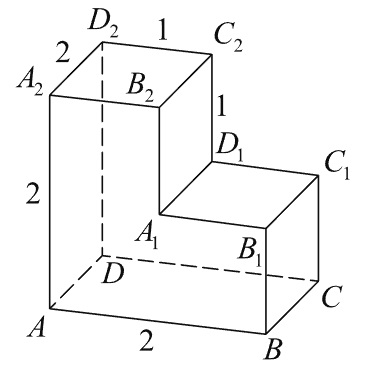
\includegraphics[align=t, width=\linewidth]{\picpath/G101M5L6-1}
		\end{minipage}
		\item С помощью этого же рисунка найдите расстояние между вершинами:
		\begin{tasks}(3)
			\task \(D\) и \(C_2\),
			\task \(B_1\) и \(D_2\),
			\task \(D_2\) и \(A_1\).
		\end{tasks}
		\item С помощью этого же рисунка найдите:
		\begin{tasks}(2)
			\task угол \( CAD_2 \),
			\task угол \( ABD \),
			\task тангенс угла \( B_2A_2C_2 \).
		\end{tasks}
		\item 
		\begin{minipage}[t]{\bodywidth}
			Построить сечение пирамиды \(ABCD\) плоскостью, проходящей через точки \(K, L, M\).
		\end{minipage}
		\hspace{0.02\linewidth}
		\begin{minipage}[t]{\picwidth}
			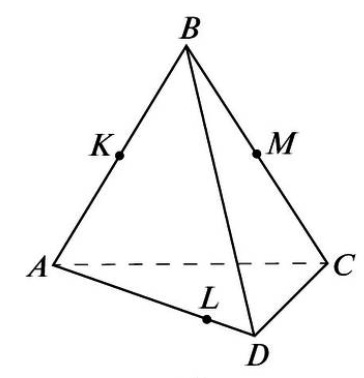
\includegraphics[align=t, width=\linewidth]{\picpath/G101M5L6-3}
		\end{minipage}
		\item Построить сечение, проходящее через центры трех соседних граней куба.
	\end{listofex}
\end{class}
%END_FOLD

%BEGIN_FOLD % ====>>_____ Занятие 7 _____<<====
\begin{class}[number=7]
	\begin{listofex}
		\item Точки \(M\) и \(N\) --- середины рёбер соответственно \(CC_1\) и \(AB\) треугольной призмы \(ABCA_1B_1C_1\). Постройте сечение призмы плоскостью, проходящей через точки \(M, N\) и \(A_1\). В каком отношении плоскость сечения делит ребро \(BC\)?
		\item Основания шестиугольной призмы \( ABCDEFA_1B_1C_1E_1F_1 \) --- правильные шестиугольники. Точка \( M \) --- середина \( BC_1 \), \( O \) --- центр грани \( ABCDEF \). Постройте сечение призмы плоскостью, проходящей через точки \( M \), \( O \) и \( E_1 \).
		\item Объем первого куба в \( 2 \) раза меньше объема второго куба. Во сколько раз площадь поверхности первого куба больше площади поверхности второго куба?
		\item Площадь грани правильного параллелепипеда равна \( 12 \). Площадь грани, перпендикулярного ей, равно \(16\). Найдите объем параллелепипеда.
		\item 
		\begin{minipage}[t]{\bodywidth}
			На рисунке изображен многогранник, все двугранные углы многогранника прямые. Найдите его объём и площадь поверхности.
		\end{minipage}
		\hspace{0.02\linewidth}
		\begin{minipage}[t]{\picwidth}
			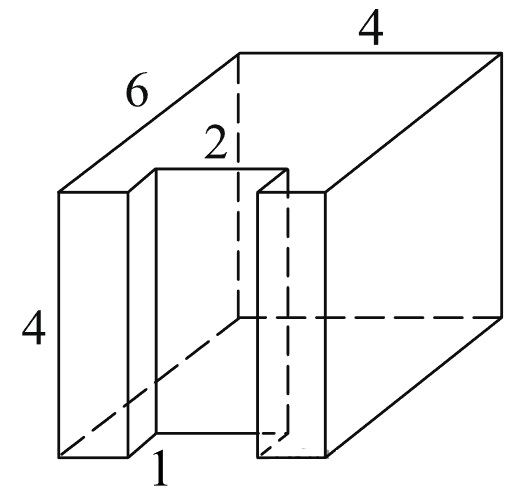
\includegraphics[align=t, width=\linewidth]{\picpath/G102M5L7-2}
		\end{minipage}
		\item 
		\begin{minipage}[t]{\bodywidth}
			На рисунке изображен многогранник, все двугранные углы многогранника прямые. Найдите его объём и площадь поверхности.
		\end{minipage}
		\hspace{0.02\linewidth}
		\begin{minipage}[t]{\picwidth}
			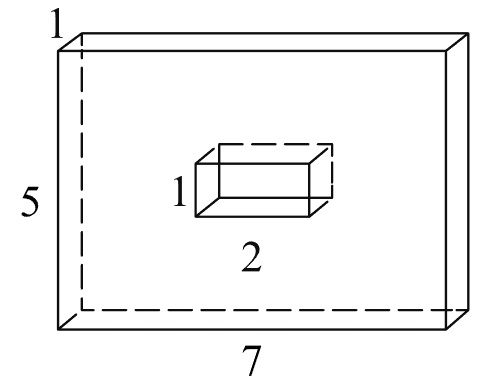
\includegraphics[align=t, width=\linewidth]{\picpath/G102M5L7-3}
		\end{minipage}
		\item Вычислить: \( \dfrac{5\cos 25\degree}{\sin 65\degree}+\dfrac{\sin 60\degree}{\cos 30\degree} \)
	\end{listofex}
\end{class}
%END_FOLD

%BEGIN_FOLD % ====>>_ Домашняя работа 1 _<<====
\begin{homework}[number=1]
	\begin{listofex}
		\item
		\begin{minipage}[t]{\bodywidth}
			На рисунке изображён график функции вида \[ f(x)=ax-|bx+c|+d, \] где числа \(a, b, c, d\) --- целые.\\ Найдите корень уравнения \(ax=d\).
		\end{minipage}
		\hspace{0.02\linewidth}
		\begin{minipage}[t]{\picwidth}
			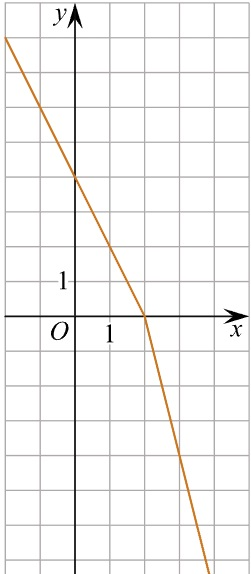
\includegraphics[align=t, width=\linewidth]{\picpath/K-L9}
		\end{minipage}
		\item Постройте сечение параллелепипеда \( ABCDA_1B_1C_1D_1 \)
		плоскостью, проходящей через следующие точки \( A \), \( C \) и середину \( C_1D_1 \).
		\item Постройте сечение треугольной пирамиды \( DABC \) плоскостью,
		проходящей через середины \( K \), \( L \) и \( M \) ребер \( AD \), \( BD \) и \( BC \).
		\item Решить равнение: \( \sqrt{\dfrac{2x+5}{3}}=5 \).
		\item Решить неравенство: \( \dfrac{x^2-x-2}{x^2-9}\ge0 \).
	\end{listofex}
\end{homework}
%END_FOLD

%BEGIN_FOLD % ====>>_ Домашняя работа 2 _<<====
\begin{homework}[number=2]
	\begin{listofex}
		\item Дана правильная шестиугольная призма \(ABCDEFA_1B_1C_1D_1E_1F_1\). Боковое ребро \(AA_1\) равно стороне основания \(ABCDEF\). Найдите углы между плоскостями: а) \(АВС\) и \(DB_1F_1\); б) \(AFF_1\) и \(DEE_1\),; в) \(AFF_1\) и \(BCC_1\), г) \(AFF_1\) и \(BDD_1\)
		\item Дана правильная шестиугольная пирамида \(SABCDEF\) с вершиной \(S\). Боковое ребро вдвое больше стороны основания. Найдите углы между плоскостями: а) \(ABC\) и \(SEF\); б) \(SBD\) и \(ABC\); в) \(SBC\) и \(SEF\); г) \(SAF\) и \(SBC\).
		\item Дана правильная четырёхугольная пирамида \(SABCD\) с вершиной \(S\). Точка \(O\) --- центр основания, \(K\) --- основание перпендикуляра, опущенного из точки \(O\) на прямую \(SC\). а) Докажите, что прямая \(OK\) перпендикулярна прямой \(BD\). б) Найдите двугранный угол при боковом ребре пирамиды, если угол между боковым ребром и плоскостью основания равен \(60 \degree \).
		\item В правильной четырёхугольной призме \(ABCDA_1B_1C_1D_1\) стороны основания равны \(2\), а боковые рёбра равны \(3\). На ребре отмечена точка \(E\) так, что \(AE:EA_1 = 1:2\). а) Постройте прямую пересечения плоскостей \(АВС\) и \(BED_1\). б) Найдите угол между плоскостями \(ABC\) и \(BED_1\).
	\end{listofex}
\end{homework}
%END_FOLD

%BEGIN_FOLD % ====>>_ Домашняя работа 3 _<<====
\begin{homework}[number=3]
	\begin{listofex}
		\item Два ребра прямоугольного параллелепипеда, выходящие из одной вершины, равны \(1, 2\). Площадь поверхности параллелепипеда равна \(16\). Найдите его диагональ.
		\item Прямоугольный параллелепипед описан около сферы с диаметром, равным \(2\) см. Найдите его объём.
		\item 
		\begin{minipage}[t]{\bodywidth}
			На рисунке изображен многогранник, все двугранные углы многогранника прямые. Найдите квадрат расстояния между вершинами \(B_2\) и \(D_3\) .
		\end{minipage}
		\hspace{0.02\linewidth}
		\begin{minipage}[t]{\picwidth}
			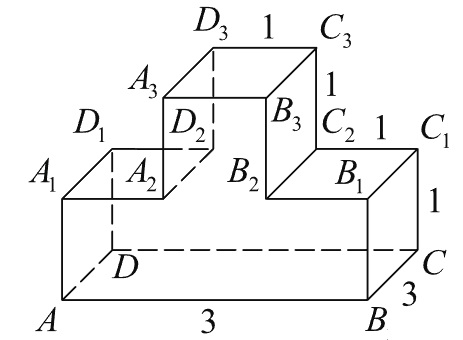
\includegraphics[align=t, width=\linewidth]{\picpath/G101M5L6-2}
		\end{minipage}
		\item С помощью этого же рисунка найдите:
		\begin{tasks}(1)
			\task расстояние между вершинами \(B\) и \(D_2\),
			\task тангенс угла \(C_2C_3B_2\).
		\end{tasks}
		\item Вычислите:
		\begin{tasks}(2)
			\task \(\dfrac{4 \cdot \sin61\degree}{\cos29\degree}\)
			\task \(\dfrac{2 \cdot \sin136\degree}{\sin68\degree \cdot \sin22\degree}\)
		\end{tasks}
	\end{listofex}
\end{homework}
%END_FOLD

%BEGIN_FOLD % ====>>_ Проверочная работа _<<====
\begin{exam}
	\begin{listofex}
		\item Вычислить:
		\begin{tasks}(3)
			\task \( \dfrac{\sqrt{2,8}\cdot\sqrt{4,2}}{\sqrt{0,24}} \)
			\task \( (49^6)^3 : (7^7)^5 \)
			\task \( \sqrt{65^2-56^2} \)
		\end{tasks}
		\item Найдите \(\dfrac{a+9b+16}{a+3b+8}\), если \(\dfrac{a}{b}=3\).
		\item Площадь грани прямоугольного параллелепипеда равна \( 15 \). Ребро, перпендикулярное этой грани, равно \(3\). Найдите объем параллелепипеда.
		\item 
		\begin{minipage}[t]{\bodywidth}
			На рисунке изображен многогранник, все двугранные углы многогранника прямые. Найдите его объём и площадь поверхности.
		\end{minipage}
		\hspace{0.02\linewidth}
		\begin{minipage}[t]{\picwidth}
			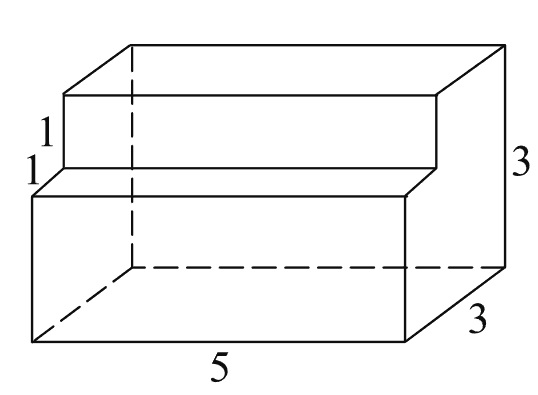
\includegraphics[align=t, width=\linewidth]{\picpath/G101M5L7-2}
		\end{minipage}
		\item 
		\begin{minipage}[t]{\bodywidth}
			На рисунке изображен многогранник, все двугранные углы многогранника прямые. Найдите его объём и площадь поверхности.
		\end{minipage}
		\hspace{0.02\linewidth}
		\begin{minipage}[t]{\picwidth}
			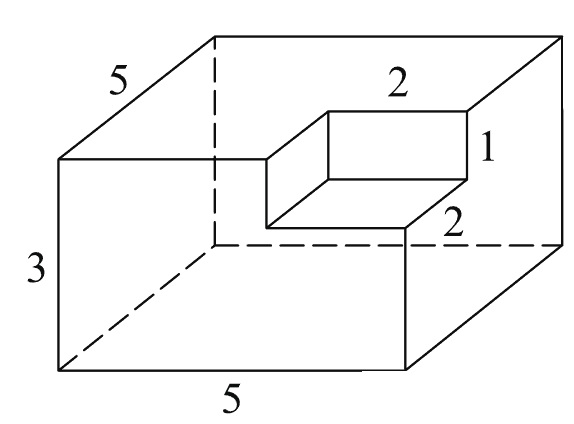
\includegraphics[align=t, width=\linewidth]{\picpath/G101M5L7-3}
		\end{minipage}
		\item
		\begin{minipage}[t]{\bodywidth}
			Постройте сечение тетраэдра плоскостью, проходящей через точки\( M, N, K\). Точка \(M\) лежит на ребре \(AD\), \(N\) --- на ребре \(DC\), \(К\) --- на ребре АВ.
		\end{minipage}
		\begin{minipage}[t]{\picwidth}
			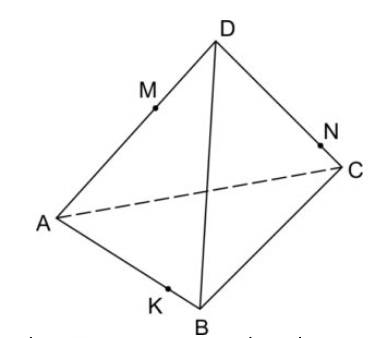
\includegraphics[align=t, width=\linewidth]{\picpath/G102M5L7-1}
		\end{minipage}
		\item Постройте сечение правильного тетраэдра \(ABCS\), проходящее через точку \(K\) --- середину ребра \(AB\), точку \(M\), делящую ребро \(AS\) в отношении \(SM:AM = 1:2\), и точку \(N\) --- середину апофемы грани \(SBC\).
		\item Два ребра прямоугольного параллелепипеда, выходящие из одной вершины, равны \(3\) и \(4\). Площадь поверхности этого параллелепипеда равна \(94\). Найдите третье ребро, выходящее из той же вершины.
		\item Три ребра прямоугольного параллелепипеда, выходящие из одной вершины, равны \(4, 6, 9\). Найдите ребро равновеликого ему куба.
	\end{listofex}
\end{exam}
%END_FOLD

%BEGIN_FOLD ====>>_ Консультация 27.12 _<<====
\begin{consultation}
	\begin{listofex}
		\item Постройте сечение треугольной пирамиды \(SABC\) плоскостью, проходящей через вершину \(B\) и середины ребер \(SA\) и \(SC\).
		\item Постройте сечение треугольной пирамиды \(SABC\) плоскостью, проходящей через вершину \(A\), середину ребра \(BS\) параллельно ребру \(BC\).
		\item  Постройте сечение треугольной пирамиды \(SABC\) плоскостью, проходящей через точку \(M\), лежащую на ребре \(AS\), точку \(N\), лежащую на ребре \(CS\), точку \(K\) лежащую на ребре \(BC\). Если \(AM:MS=1:2\), \(SN:NC=1:2\), \(BK:KC=1:2\)
		\item  Постройте сечение параллелепипеда \(ABCDA_1B_1C_1D_1\) плоскостью, проходящей середины рёбер \(A_1B_1\), \(CC_1\) и вершину \(A\).
		\item Основание пирамиды \(SABCD\) — параллелограмм \(ABCD\). Постройте сечение пирамиды плоскостью, проходящей середину ребра \(SA\) и точки \(M\) и \(N\) рёбер \(SB\) и \(SC\), если \(BM:MS=SN:NC =1:3\).
		\item  Основания шестиугольной призмы \(ABCDEF\) и \(A_1B_1C_1E_1F_1\) --- правильные шестиугольники. Точка \(M\) --- середина ребра \(CC_1\), \(O\) --- центр грани \(ABCDEF\). Постройте сечение призмы плоскостью, проходящей через точки \(M\), \(O\) и \(E_1\).
		\item  Дана правильная четырёхугольная пирамида \(SABCD\) с вершиной \(S\). Точки \(M\) и \(N\) —середины рёбер \(AB\) и \(SC\). Постройте сечение пирамиды плоскостью, проходящей через прямую \(MN\) параллельно \(SA\).
		\newpage
		
		\item Решить уравнение:
		\begin{tasks}(2)
			\task \( \sin x = \dfrac{1}{2} \)
			\task \( \cos x = -1 \)
			\task \( 2\sin x = -\sqrt{2} \)
			\task \( 3\tg x = \sqrt{3} \)
			\task \( \sin^2 x = \dfrac{1}{2} \)
		\end{tasks}
		\item Решить неравенство:
		\begin{tasks}(2)
			\task \( \sin x > \dfrac{1}{2} \)
			\task \( \cos x \le \dfrac{\sqrt{2}}{2} \)
			\task \( \sin x < 1 \)
			\task \( \sin x \ge -\dfrac{3}{2}\)
		\end{tasks}
	\end{listofex}
\end{consultation}
%END_FOLD

%BEGIN_FOLD ====>>_ Консультация 27.01 _<<====
\begin{consultation}
	\begin{listofex}
		\item  Решите уравнение \( \sin\left( 2x-\dfrac{\pi}{3} \right)=\dfrac{\sqrt{3}}{2} \)
		\item  Решите уравнение \( \ctg\left( 3x-\dfrac{\pi}{6} \right)=\sqrt{3} \)
		\item  Решите уравнение \( \sin^2x-\sin x=0 \)
		\item  Решите уравнение \( 5\tg^2x+6\tg x+1=0 \)
		\item  Решите уравнение \( \cos^2x=\dfrac{1}{4} \)
		\item  Решите уравнение \( \cos {\left(x - \dfrac{3\pi}{2}\right)} = \sin 2x \)
		\item  Решите уравнение \( 8\sin x + 4\cos^2 x = 7 \)
		\item  Решите уравнение \( \tg x-2\ctg x=1 \)
		\item  Решите уравнение \( \sqrt{2}\cos {(\pi-x)} + 2\cos^2{(\pi+x)}=0 \)
		\item  Решите уравнение \( 4\cos^4 x - 15\cos 2x -1= 0 \)
	\end{listofex}
\end{consultation}
%END_FOLD

%BEGIN_FOLD ====>>_ Консультация 27.01 _<<====
\begin{consultation}
	\begin{listofex}
		\item 
		\begin{minipage}[t]{\bodywidth}
			На рисунке изображен многогранник, все двугранные углы многогранника прямые. Найдите его объём и площадь поверхности.
		\end{minipage}
		\hspace{0.02\linewidth}
		\begin{minipage}[t]{\picwidth}
			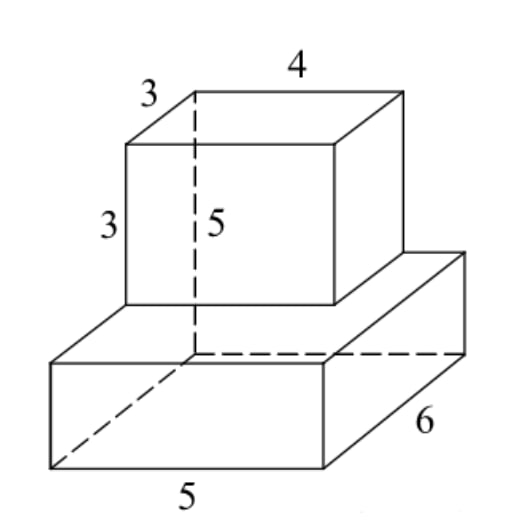
\includegraphics[align=t, width=\linewidth]{\picpath/G102M5Cons-1}
		\end{minipage}
	\item 
	\begin{minipage}[t]{\bodywidth}
		На рисунке изображен многогранник, все двугранные углы многогранника прямые. Найдите его объём и площадь поверхности.
	\end{minipage}
	\hspace{0.02\linewidth}
	\begin{minipage}[t]{\picwidth}
		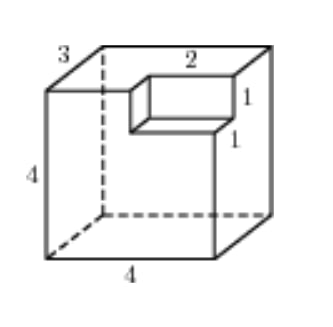
\includegraphics[align=t, width=\linewidth]{\picpath/G102M5Cons-2}
	\end{minipage}
	\item Вычислить:
	\begin{enumcols}[itemcolumns=3]
		\item \exercise{562}
		\item \exercise{564}
		\item \exercise{569}
		\item \exercise{571}
		\item \exercise{579}
	\end{enumcols}
	\item Вычислить:
	\begin{enumcols}[itemcolumns=3]
		\item \exercise{1577}
		\item \exercise{1578}
		\item \exercise{1579}
	\end{enumcols}
	\item Вычислить:
	\begin{enumcols}[itemcolumns=3]
		\item \exercise{1572}
		\item \exercise{1565}
		\item \exercise{1566}
		\item \exercise{1573}
		\item \exercise{1567}
		\item \exercise{1575}
		\item \exercise{1594}
	\end{enumcols}
	\end{listofex}
\end{consultation}
%END_FOLD